\documentclass[11pt]{article}
\usepackage{graphicx}
\usepackage{hyperref}
\usepackage{appendix}
\usepackage{amsmath}
\usepackage{amsthm}
\usepackage{amssymb}
\usepackage{float}
\usepackage{multirow}
\usepackage{commath}
\usepackage{booktabs}
\usepackage{subcaption}
\renewcommand{\arraystretch}{1.2}
\usepackage{siunitx}
\sisetup{detect-all}
\usepackage{listings}
\usepackage{color} %red, green, blue, yellow, cyan, magenta, black, white
\definecolor{mygreen}{RGB}{28,172,0} % color values Red, Green, Blue
\definecolor{mylilas}{RGB}{170,55,241}
\usepackage[a4paper,margin=20mm]{geometry}
\numberwithin{equation}{section}
\setlength{\parskip}{\baselineskip}
\setlength{\parindent}{0pt}
\hypersetup{
    colorlinks=true,
    linkcolor=black,
    filecolor=black,      
    urlcolor=black,
    citecolor=black
}
\urlstyle{same}
\begin{document}
\title{\textbf{UCL Mechanical Engineering 2021/2022}\\MECH0026 Coursework One}
\author{Hasha Dar}
\date{\today}
\maketitle
\tableofcontents
\listoffigures
\section{Description of the finite element model setup}
\subsection{Geometry of the plate}
We are to model the stresses in the vicinity of a hole in an infinite plate. As we cannot physically model an infinite plate, we must bound our plate to finite dimensions. Our plate is also symmetrical along the $x$- and $y$- axes, hence we can model a quarter of the plate and extend our analysis to the other sections. The plate in this analysis has the geometry shown in Figure \ref{plateGeo}.
\begin{figure}[H]
    \centering
    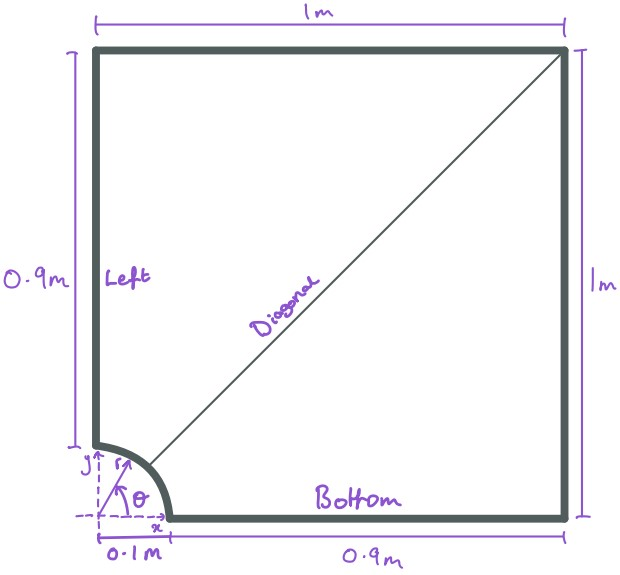
\includegraphics[width = 0.6\textwidth]{./img/diagram5.jpg}
    \caption{Geometry of the plate.}
    \label{plateGeo}
\end{figure}
The material of our plate is given as a generic aluminium alloy, with material properties $E = \SI{70}{\giga\pascal}$ and $v = 0.33$. 
\subsection{Boundary conditions}
The plate is subject to a biaxial load along the edges of the plate. The forces are shown in Figure \ref{plateLoading}. The stress biaxiality ratio in this case is 2.5. The values for $\sigma_1$ and $\sigma_2$ were chosen as -1000 and -400 in ABAQUS, to simulate a tension force fulfilling the biaxiality ratio. 
\begin{figure}[H]
    \centering
    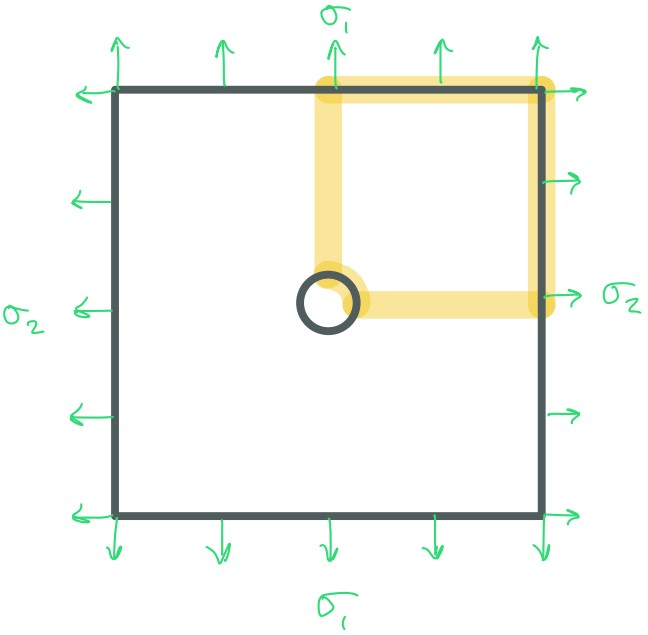
\includegraphics[width = 0.5\textwidth]{./img/diagram6.jpg}
    \caption{Loading of the plate.}
    \label{plateLoading}
\end{figure}
\subsection{Element type and justification of choice}
Since we are looking at a plate undergoing stresses in the $x$- and $y$- directions, we can model the plate in a 2D configuration. We can assume the plate to be thin as when the plate extends to infinity, its relative thickness becomes almost negligible. Our loads are only in the $x$- and $y$- directions with our three stress tensors in the $z$- direction being 0. Plane strain is not applicable in this situation as we are not analysing a thick component. 
\subsection{Mesh configuration}
Nine different mesh configurations were trialled and the data saved for each. Linear Quad and Tri and Quadratic Quad and Tri were all tested with seed sizes of 0.01 and 0.05. Using MATLAB, the S22 data from the 'left' path (defined as the vertical left side of the plate) was plotted.
\begin{figure}[H]
    \centering
    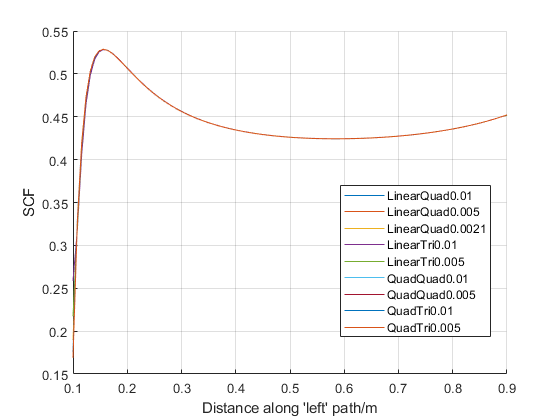
\includegraphics[width = 0.7\textwidth]{./img/diagram1.png}
    \caption{Left side $\frac{\sigma_{\theta\theta}}{\sigma_1}$ - $r$ plots for each mesh configuration.}
    \label{meshconfig}
\end{figure}
As our geometry is quite simple, Tri meshes showed to be no more efficient in creating effective meshes, with extremely similar values for the same configurations (changing only from Quad to Tri). As our plate is nearly square in shape, Quad meshing is desirable. Decreasing seed size showed to converge our value. In Figure \ref{meshconfig}, we see that each mesh configuration leads to very similar output. However, Quadratic Quad with a seed size of 0.005 showed to converge to the lowest value and was used for this analysis. 
\section{Post-processing and examination of results}
\subsection{Analytical calculation of stress field}
Let us analyse a case of uniaxial tension and use the concept of superposition to find our stress distribution.

The biharmonic equation written in polar coordinates is:
\begin{gather}
    \left(\dfrac{\partial^2}{\partial r^2} + \dfrac{1}{r}\dfrac{\partial}{\partial r}+\dfrac{1}{r^2}\dfrac{\partial^2}{\partial \theta^2}\right)\left(\dfrac{\partial^2\phi}{\partial r^2}+\dfrac{1}{r}\dfrac{\partial\phi}{\partial r}+\dfrac{1}{r^2}\dfrac{\partial^2 \phi}{\partial\theta^2}\right) = 0
\end{gather}
We know our boundary conditions which are:
\begin{gather}
    \sigma_r, \, \tau_{r\theta} = 0, \, r = a\\
    \dfrac{\sigma_y}{\sigma_x} \rightarrow 2.5; \, r \rightarrow \infty\\
    \tau_{xy} \rightarrow 0; \, r \rightarrow \infty
\end{gather}
We can use separation of variables to obtain a solution of the form:
\begin{gather}
    \phi = R(r)\Theta (\theta)
\end{gather}
One solution is:
\begin{gather}
    \phi = \left(Ar^2 + Br^4 \dfrac{C}{r^2} + D\right)\cos \left(2\theta\right)\label{airy1}
\end{gather}
Let us also consider:
\begin{align}
    \phi = A \ln r + Cr^2 \label{airy2}
\end{align}
A linear combination of \ref{airy1} and \ref{airy2} yields a stress function that can be shown to represent the stress distribution in a large plate with a circular hole subjected to a uniform tensile stress $\sigma$. By inputting our boundary conditions we can come to the following stress function:
\begin{gather}
    \phi = \dfrac{\sigma}{2}\left(2r^2 - a^2 \ln r\right) - \dfrac{\sigma}{4}\left(r^2+\dfrac{a^4}{r^2}-2a^2\right)\cos \left(2\theta\right)
\end{gather}
Now we can find our stresses:
\begin{gather}
    \sigma_r = \dfrac{1}{r}\dfrac{\partial \phi}{\partial r} + \dfrac{1}{r^2}\dfrac{\partial^2\phi}{\partial \theta^2} = \dfrac{\sigma}{2}\left(1 - \dfrac{a^2}{r^2}\right) + \dfrac{\sigma}{2}\left(1+\dfrac{3a^4}{r^4}-\dfrac{4a^2}{r^2}\right)\cos\left(2\theta\right)\\
    \sigma_{\theta} = \dfrac{\partial^2\phi}{\partial r^2} = \dfrac{\sigma}{2}\left(1 + \dfrac{a^2}{r^2}\right) - \dfrac{\sigma}{2}\left(1 + \dfrac{3a^4}{r^4}\right)\cos \left(2\theta\right)\\
    \tau_{r\theta} = -\dfrac{\partial}{\partial r}\left(\dfrac{1}{r}\dfrac{\partial \phi}{\partial \theta}\right) = -\dfrac{\sigma}{2}\left(1 - \dfrac{3a^4}{r^4}+\dfrac{2a^2}{r^2}\right)\sin\left(2\theta\right)
\end{gather}
Superimposing a tensile stress at a \SI{90}{\degree} angle simply involves adding a $\dfrac{\pi}{2}$ term to our $\theta$ components. Let us denote the stress in the vertical direction as $\sigma_y$ and the stress in the horizontal direction as $\sigma_x$:
\begin{multline}
    \sigma_{rr} = \dfrac{\sigma_x}{2}\left(1 - \dfrac{a^2}{r^2}\right) + \dfrac{\sigma_x}{2}\left(1+\dfrac{3a^4}{r^4}-\dfrac{4a^2}{r^2}\right)\cos\left(2\theta\right) + \\\dfrac{\sigma_y}{2}\left(1 - \dfrac{a^2}{r^2}\right) + \dfrac{\sigma_y}{2}\left(1+\dfrac{3a^4}{r^4}-\dfrac{4a^2}{r^2}\right)\cos\left(2\left(\theta + \dfrac{\pi}{2}\right)\right)
\end{multline}
\begin{multline}
    \sigma_{\theta\theta} = \dfrac{\sigma_x}{2}\left(1 + \dfrac{a^2}{r^2}\right) - \dfrac{\sigma_x}{2}\left(1 + \dfrac{3a^4}{r^4}\right)\cos \left(2\theta\right) + \\ \dfrac{\sigma_y}{2}\left(1 + \dfrac{a^2}{r^2}\right) - \dfrac{\sigma_y}{2}\left(1 + \dfrac{3a^4}{r^4}\right)\cos \left(2\left(\theta + \dfrac{\pi}{2}\right)\right)
\end{multline}
\begin{gather}
    \tau_{r\theta} = -\dfrac{\sigma_x}{2}\left(1 - \dfrac{3a^4}{r^4}+\dfrac{2a^2}{r^2}\right)\sin\left(2\theta\right) -\dfrac{\sigma_y}{2}\left(1 - \dfrac{3a^4}{r^4}+\dfrac{2a^2}{r^2}\right)\sin\left(2\left(\theta + \dfrac{\pi}{2}\right)\right)
\end{gather}
Simplifying and inputting our boundary conditions:
\begin{gather}
    \sigma_{rr} = \dfrac{\sigma_x + \sigma_y}{2}\left(1 - \dfrac{a^2}{r^2}\right) + \dfrac{\sigma_x + \sigma_y}{2}\left(1 + \dfrac{3a^4}{r^4}- \dfrac{4a^2}{r^2}\right)\cos \left(2\theta\right)\\
    \sigma_{\theta\theta} = \dfrac{\sigma_x + \sigma_y}{2}\left(1 + \dfrac{a^2}{r^2}\right) - \dfrac{\sigma_x - \sigma_y}{2}\left(1 + \dfrac{3a^4}{r^4}\right)\cos\left(2\theta\right)\\
    \tau_{r\theta} = \dfrac{\sigma_y - \sigma_x}{2}\left(1 -\dfrac{3a^4}{r^4}+ \dfrac{2a^2}{r^2}\right)\sin\left(2\theta\right)
\end{gather}
At $r =a$:
\begin{gather}
    \sigma_{rr} = 0\\
    \sigma_{\theta\theta} = \sigma_x + \sigma_y - 2\left(\sigma_x - \sigma_y\right)\cos\left(2\theta\right)\\
    \tau_{r\theta} = 0
\end{gather}
$\sigma_{\theta}$ takes a maximum value at $\theta = \dfrac{\pi}{2}$ and $\dfrac{3\pi}{2}$:
\begin{gather}
    \sigma_{max} = 3\sigma_x - \sigma_y\label{sigmaMax}
\end{gather}
\subsection{Distribution of the three components of the stress field in the plate from the FE analysis}
After submitting the data for analysis in ABAQUS, the following results were achieved.
\begin{figure}[H]
    \centering
    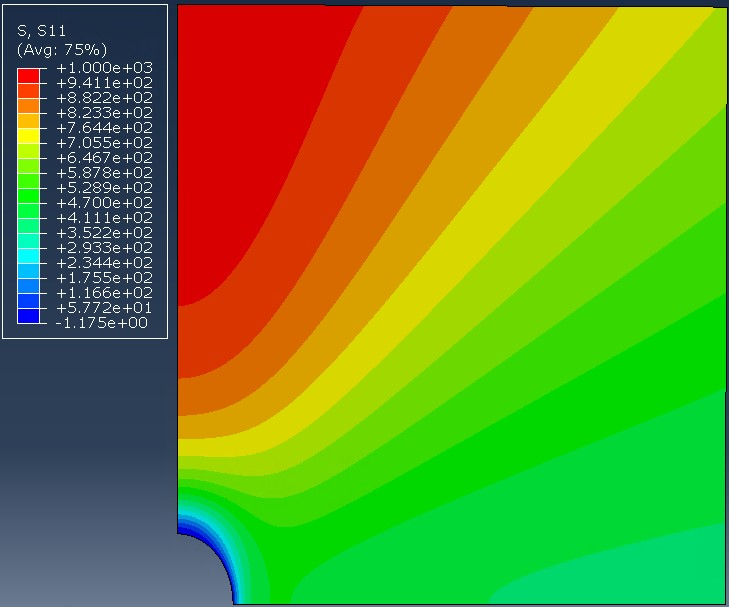
\includegraphics[width = 0.5\textwidth]{./img/diagram2.jpg}
    \caption{S11 output from ABAQUS.}
\end{figure}
\begin{figure}[H]
    \centering
    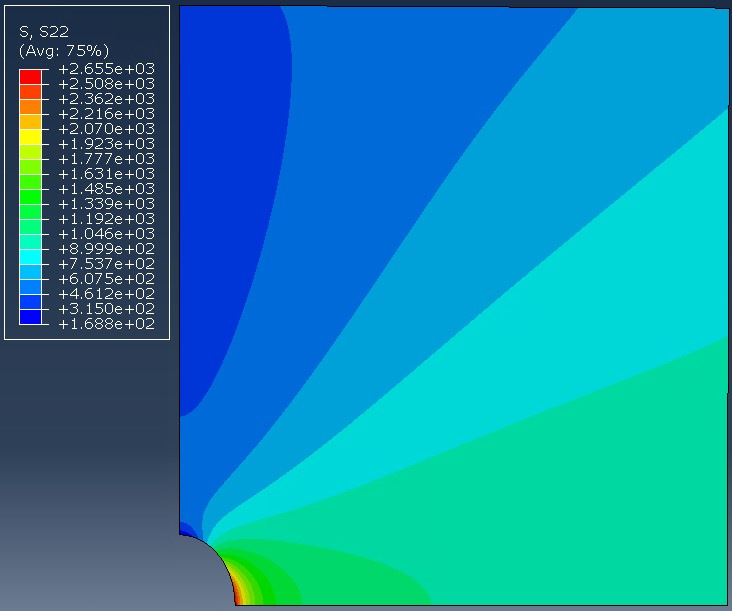
\includegraphics[width = 0.5\textwidth]{./img/diagram3.jpg}
    \caption{S22 output from ABAQUS.}
\end{figure}
\begin{figure}[H]
    \centering
    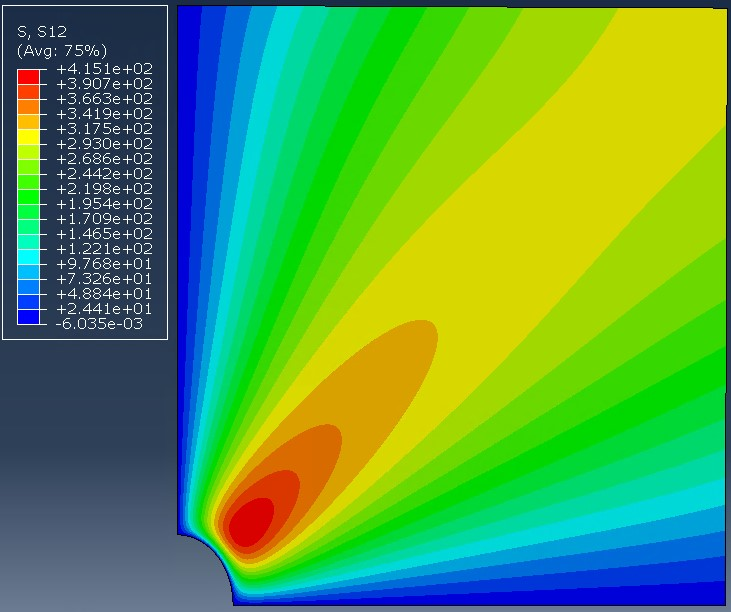
\includegraphics[width = 0.5\textwidth]{./img/diagram4.jpg}
    \caption{S12 output from ABAQUS.}
\end{figure}
\subsection{Plots of SCF from the FE analysis}
MATLAB was used to plot $\frac{\sigma_{rr}}{\sigma_1} - r$, $\frac{\sigma_{\theta\theta}}{\sigma_1}-r$ and $\frac{\tau_{r\theta}}{\sigma_1}-r$ for $\theta = 0, \, \frac{\pi}{4}$ and $\frac{\pi}{2}$.
\begin{figure}[H]
    \centering
    \begin{minipage}{.5\textwidth}
      \centering
      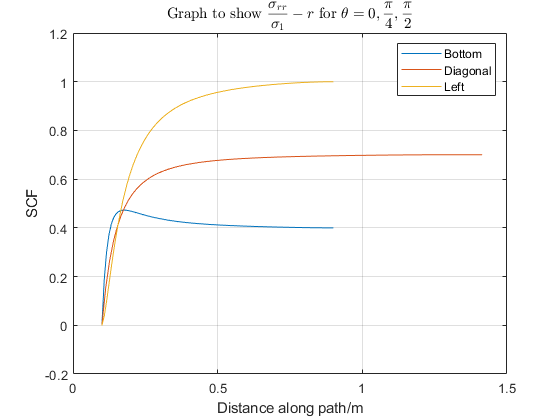
\includegraphics[width=\linewidth]{./img/diagram7.png}
      \captionof{figure}{Plot of $\frac{\sigma_{rr}}{\sigma_1}-r$ for $\theta = 0, \frac{\pi}{4}, \frac{\pi}{2}$.}
      \label{fig:sigmarr}
    \end{minipage}%
    \begin{minipage}{.5\textwidth}
      \centering
      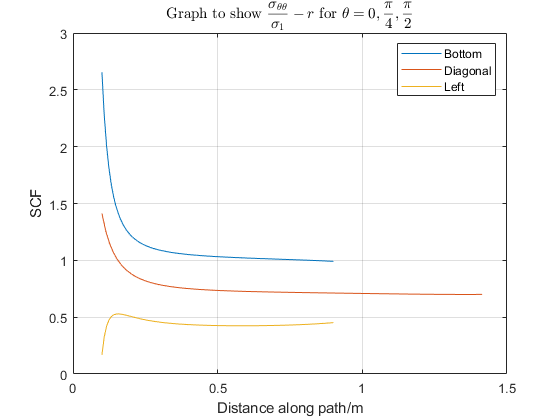
\includegraphics[width=\linewidth]{./img/diagram8.png}
      \captionof{figure}{Plot of $\frac{\sigma_{\theta\theta}}{\sigma_1}-r$ for $\theta = 0, \frac{\pi}{4}, \frac{\pi}{2}$.}
      \label{fig:sigmathetatheta}
    \end{minipage}
\end{figure}
\begin{figure}[H]
    \centering
    \begin{minipage}{.33\textwidth}
      \centering
      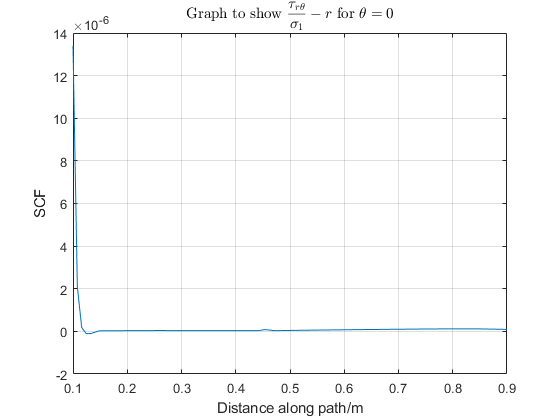
\includegraphics[width=\linewidth]{./img/diagram9.png}
      \captionof{figure}{Plot of $\frac{\tau_{r\theta}}{\sigma_1}-r$ for $\theta = 0$.}
      \label{fig:taurtheta0}
    \end{minipage}%
    \begin{minipage}{.33\textwidth}
        \centering
        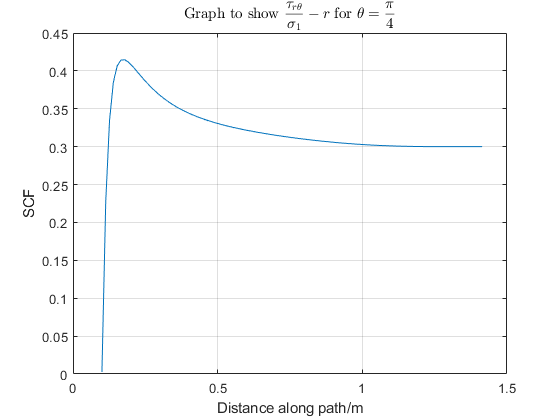
\includegraphics[width=\linewidth]{./img/diagram10.png}
        \captionof{figure}{Plot of $\frac{\tau_{r\theta}}{\sigma_1}-r$ for $\theta = \frac{\pi}{4}$.}
        \label{fig:taurthetapi4}
      \end{minipage}%
    \begin{minipage}{.33\textwidth}
      \centering
      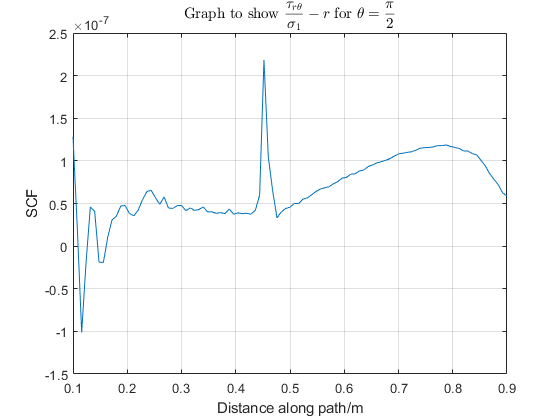
\includegraphics[width=\linewidth]{./img/diagram11.png}
      \captionof{figure}{Plot of $\frac{\tau_{r\theta}}{\sigma_1}-r$ for $\theta = \frac{\pi}{2}$.}
      \label{fig:taurthetapi2}
    \end{minipage}
\end{figure}
\section{Discussion}
\subsection{Location and magnitude of maximum SCF.}
Looking at our ABAQUS field data, we can see that the maximum SCF occurs at the hole boundary on the bottom side. Looking at \ref{sigmaMax} and inputting our load values, we get:
\begin{gather}
    \frac{\sigma_{max}}{1000} = \frac{3(1000)-400}{1000} = 2.6 
\end{gather}
This aligns with the plot in Figure \ref{fig:sigmathetatheta}, where we see the maximum SCF approximately reaching 2.6. We see a discrepancy in the value with an error of 0.055, when comparing the ABAQUS data and the analytical solution. This may be due to the mesh sizing and due to the fact that we have modelled our plate as finite. 
\appendix
\section{MATLAB code}
\lstset{language=Matlab,%
    %basicstyle=\color{red},
    breaklines=true,%
    morekeywords={matlab2tikz},
    keywordstyle=\color{blue},%
    morekeywords=[2]{1}, keywordstyle=[2]{\color{black}},
    identifierstyle=\color{black},%
    stringstyle=\color{mylilas},
    commentstyle=\color{mygreen},%
    showstringspaces=false,%without this there will be a symbol in the places where there is a space
    numbers=left,%
    numberstyle={\tiny \color{black}},% size of the numbers
    numbersep=9pt, % this defines how far the numbers are from the text
    emph=[1]{for,end,break},emphstyle=[1]\color{red}, %some words to emphasise
    %emph=[2]{word1,word2}, emphstyle=[2]{style},    
}
\lstinputlisting{./MCode/AbaqusData.m}
\end{document}